\documentclass[a4paper,11pt]{uzreport}
\author{
  Erwin Konkel\\
  Mateusz Znojek\\
  Stanisław Mól - Scrum Master\\
}
\group{33INF-SSI-SP/B}
\class{Część teoretyczna}
\labnumber{Zaawansowane technologie usług sieciowych}
\date{20.01.2021}
\supervisor{dr inż. Piotr Powroźnik}

\begin{document}
  \maketitle
  
\section{Opis systemu}
	System przeznaczony do nakładania planu zajęć Uniwersytetu Zielonogórskiego na czytelną siatkę, na wzór do kalendarza google. Użytkownik ma możliwość wyboru kierunku, grupy oraz podgrupy, względem której ma zostać zmapowany plan. Informacje te zostaną zapamiętane dla zalogowanego użytkownika.
    
    \begin{itemize}[leftmargin=0.50in]

        \item Grupą docelową systemu są studenci Uniwersytetu Zielonogórskiego.


    
    \end{itemize}

\section{Opis istniejących rozwiązań}
	Najszerzej znanym rozwiązaniem jest "G Suit" działający w chmurze obliczeniowej pakiet zwiększający produktywność oraz oprogramowanie do pracy grupowej i oprogramowanie oferowane przez Google na zasadzie subskrypcji. Na jego podstawie można wywnioskować, że czytelność planu odgrywa główną rolę i właśnie na tym aspekcie zostanie skupiony porojekt. Głównym elementem na którym wzorowany będzie cały projekt jest kalendarz google.

    \begin{figure}[ht!]
        \centering
        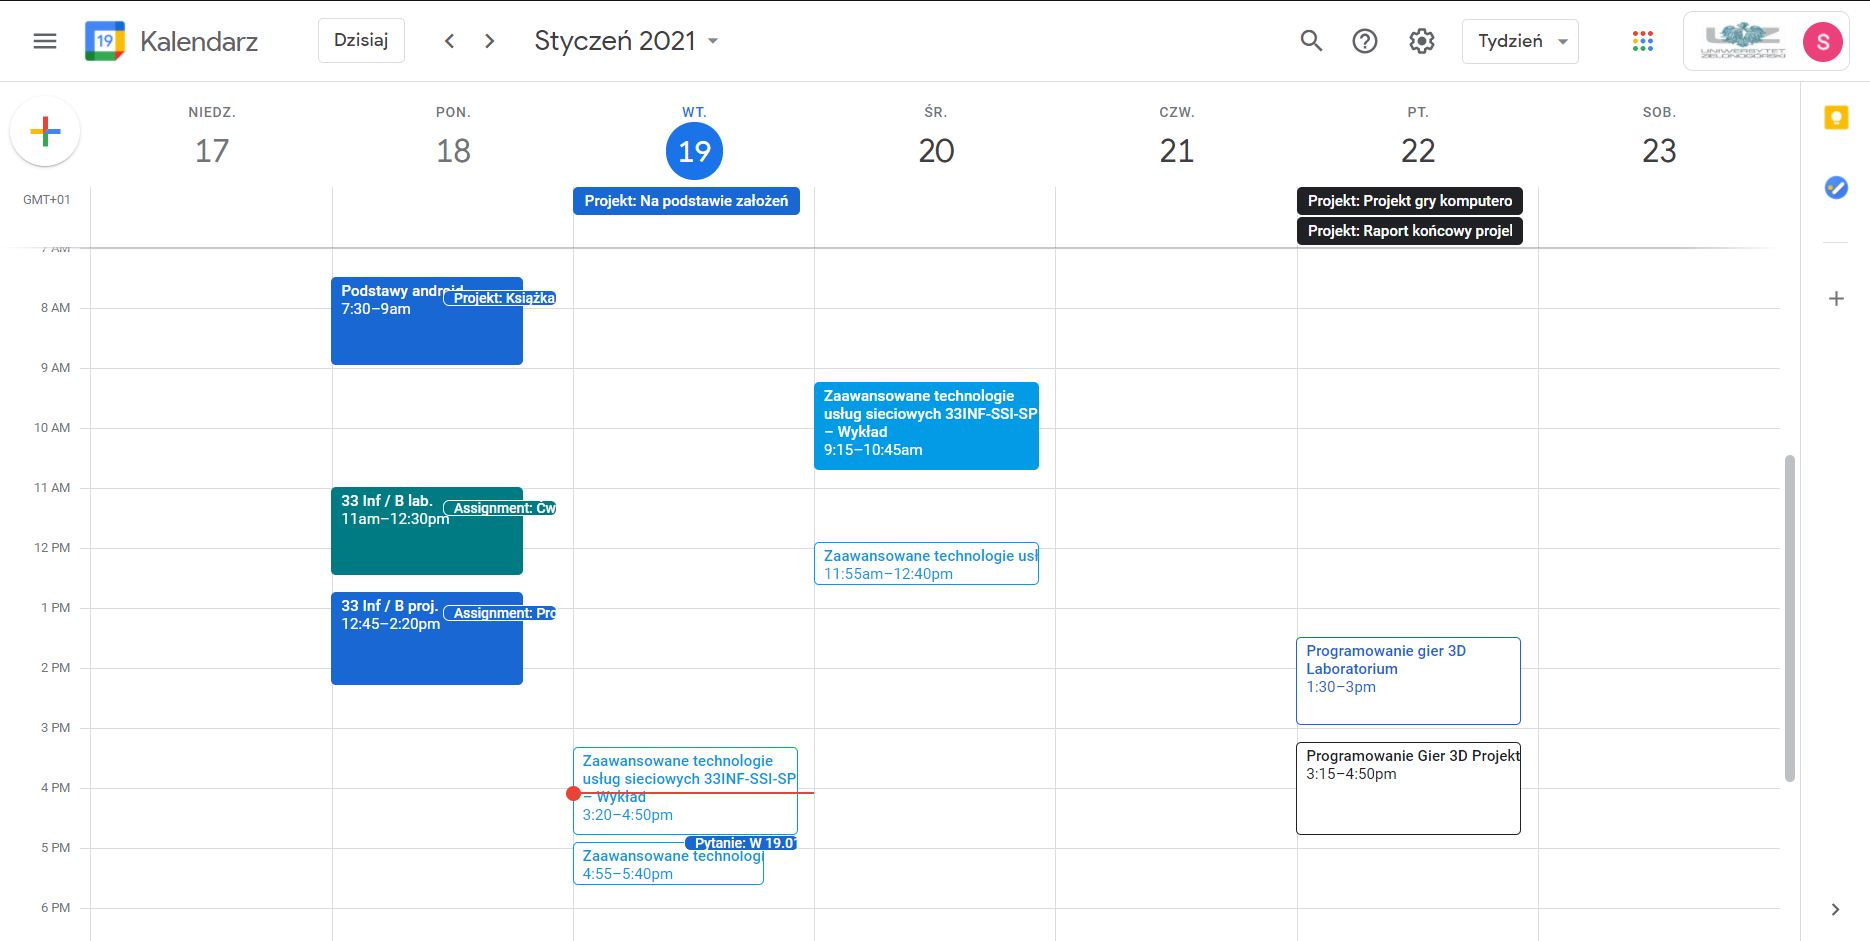
\includegraphics[width=6in]{pictures/Kalendarz-Google_1.jpg}
        \caption{Kalendarz Google}
        \label{fig2}
     \end{figure}

\section{Opis problemów}
	Główne problemy przewidziane podczas projektowania, oraz proponowane rozwiązania:

	\begin{itemize}[leftmargin=0.5in]
            
		\item Przechowywanie danych użytkowników w bazie - jednym z problemów będzie przechowywanie danych wrażliwych takich jak hasła - 			 			rozwiązaniem tego problemu będzie przechowywanie zahashowanych danych.
                
 	\end{itemize}

\section{Diagram bazy danych i relacji}
    Diagram bazy danych prezentuje się jak na rysunku \ref{fig11}. Trzonem łączącym grupy jest grupa, która posiada najważniejsze relacje łączące studenta z danymi o konkretnych zajęciach. 
    \begin{figure}[ht!]
        \centering
        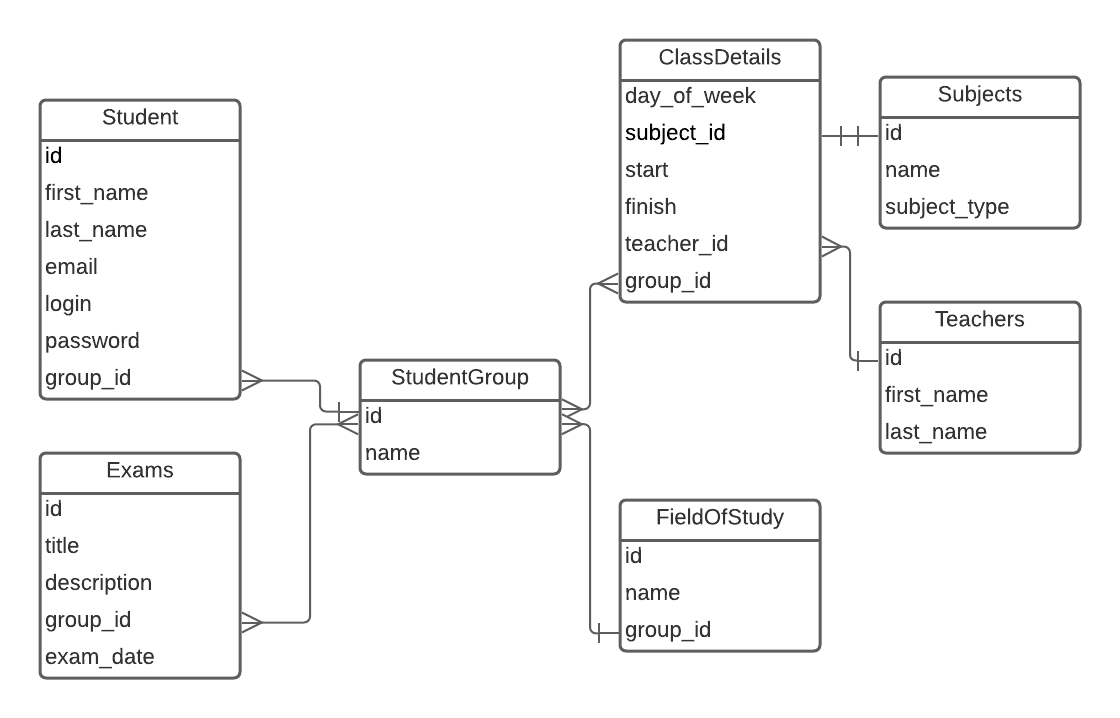
\includegraphics[width=6in]{pictures/UZplaner-baza-danych.png}
        \caption{Diagram bazy danych}
        \label{fig11}
     \end{figure}

\section{Diagram użycia}
    Diagram użycia prezentuje sie jak na rysunku \ref{fig3}. Prezentuje on podstawowe funkcjonalności na których się skupiliśmy w budowie tej platformy tj. wyświetlanie odpowiednio sformatowanej tabeli z zajęciami konkretnej grupy lub zarejestrowanego użytkownika
    \begin{figure}[ht!]
        \centering
        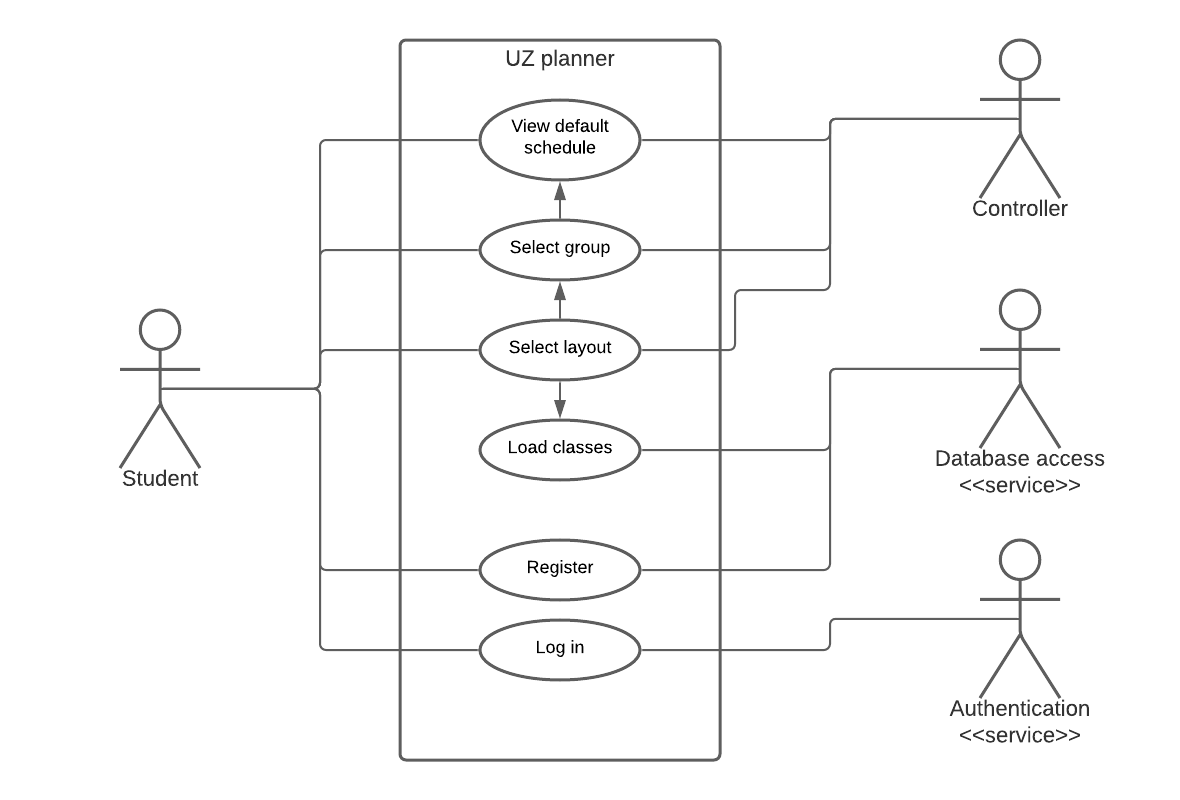
\includegraphics[width=6in]{pictures/use_case.png}
        \caption{Diagram użycia (\textit{Use Case})}
        \label{fig3}
     \end{figure}

\section{Tabele przypadków użycia}
    Tabele przypadków użycia to kolejno dla każdej funkcjonalności: rejestracja rysunek \ref{fig4}, logowanie rysunek \ref{fig5}, zmiana danych użytkownika rysunek \ref{fig6}, wyświetlanie głównego widoku planu rysunek \ref{fig7}, wybieranie grupy rysunek \ref{fig8}, wybieranie układu widoku planu rysunek \ref{fig9}
    \begin{figure}[ht!]
        \centering
        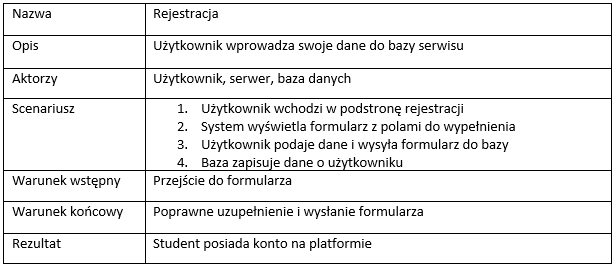
\includegraphics[width=6in]{pictures/rejestracja.PNG}
        \caption{Tabela rejestracji}
        \label{fig4}
     \end{figure}
     \begin{figure}[ht!]
        \centering
        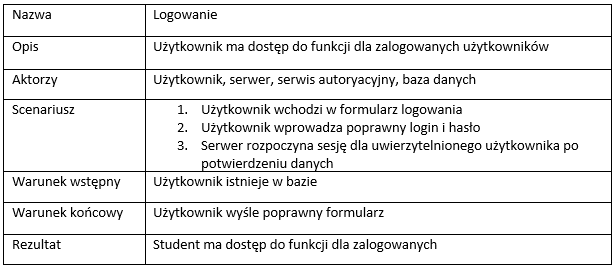
\includegraphics[width=6in]{pictures/logowanie.PNG}
        \caption{Tabela logowania}
        \label{fig5}
     \end{figure}
     \begin{figure}[ht!]
        \centering
        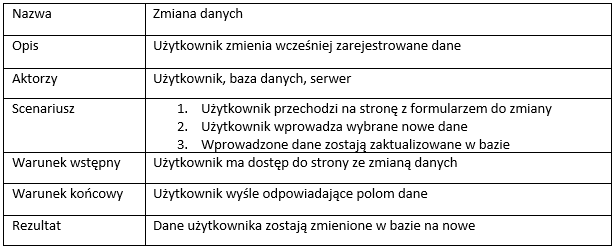
\includegraphics[width=6in]{pictures/zmiana danych.PNG}
        \caption{Tabela zmiany danych}
        \label{fig6}
     \end{figure}
     \begin{figure}[ht!]
        \centering
        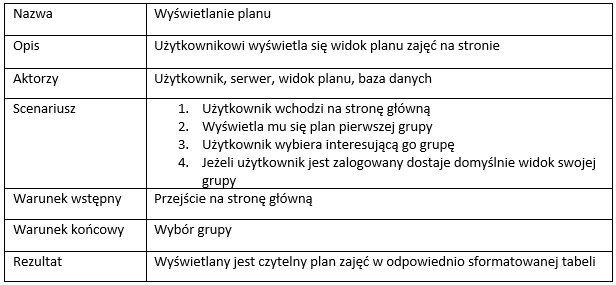
\includegraphics[width=6in]{pictures/wyswietlanie planu.PNG}
        \caption{Tabela wyświetlania planu}
        \label{fig7}
     \end{figure}
     \begin{figure}[ht!]
        \centering
        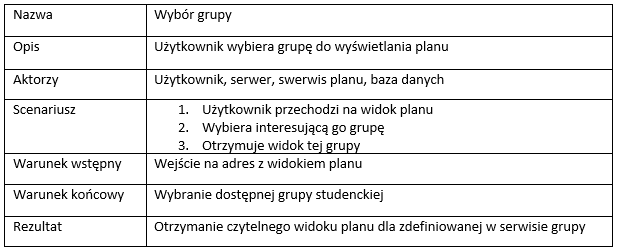
\includegraphics[width=6in]{pictures/wybor grupy.PNG}
        \caption{Tabela wyboru grupy}
        \label{fig8}
     \end{figure}
     \begin{figure}[ht!]
        \centering
        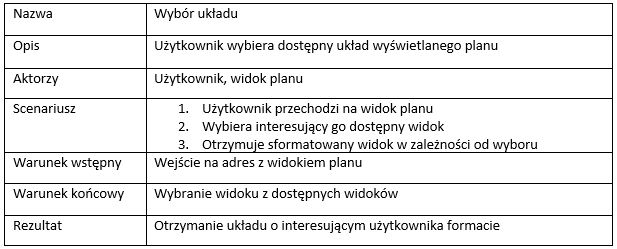
\includegraphics[width=6in]{pictures/wybor ukladu.PNG}
        \caption{Tabela wyboru układu}
        \label{fig9}
     \end{figure}


\section{Diagram komponentów/obiektów}



\section{Diagram funkcjonalny/strukturalny}


    
\clearpage
\section{Funkcjonalności}
    \begin{itemize}[leftmargin=0.50in]
    
     \item \textbf{Niezalogowany użytkownik:}
            \begin{itemize}[leftmargin=0.25in]
            
                \item logowanie / rejestracja

                \item wybór grupy dziekańskiej bez możliwości zapamiętania wyboru
                
                \item podgląd planu zajęć wybranej grupy dziekańskiej
                
                \item wybór motywu
                
            \end{itemize}

     \item \textbf{Zalogowany użytkownik:}
            \begin{itemize}[leftmargin=0.25in]
            
                \item wylogowanie

                \item wybór grupy dziekańskiej z możliwością zapamiętania wyboru
                
                \item podgląd swojego planu
                
                \item możliwość dodania informacji o kolokwium do zajęć
                
                \item możliwość dodania własnego zdarzenia
                
                \item wysłanie powiadomienia e-mail z przypomnieniem
                
                \item wyszukiwanie wykładowcy
                
                \item wybór motywu
                
                \item edycja zdarzeń zawartych w kalendarzu
                
                \item tablica TODO
     
            \end{itemize}
     
    \end{itemize}
    
\clearpage
\section{Opis funkcjonalności}
    
    \begin{itemize}[leftmargin=0.50in]
    
        \item \textbf{Rejestracja / Logowanie / Wylogowanie} - prosta funkcjonalność pozwalająca na zarejestrowanie się użytkownika, następnie autoryzację na podstawie podanego loginu i hasła, oraz wylogowanie po zakończonej sesji.
        
        \item \textbf{Wybór grupy dziekańskiej} - użytkownik niezalogowany będzie miał możliwość wyboru grupy i podglądu planu zajęć dla danej grupy, jednakże nie będzie miał możliwości zapamiętania tego wyboru. Dla użytkownika zalogowanego będzie istniała możliwość zapamiętania wybranej grupy, początkowo wybór ten będzie możliwy podczas rejestracji, lecz będzie można zmienić wybór w panelu użytkownika.
        
        \item \textbf{Podgląd planu} - plan będzie wyświetlany w czytelnej formie, dzięki nałożeniu na siatkę czasu (podobnie jak w kalendarzu google).
        
        \item \textbf{Dodanie informacji o kolokwium do zajęć} - zalogowany użytkownik będzie miał możliwość dodania informacji czy na danych zajęciach zaplanowane jest kolokwium.
        
        \item \textbf{Dodanie własnego zdarzenia} - zalogowany użytkownik ma możliwość dodania własnego zdarzenia.
        
        \item \textbf{Wysłanie powiadomienia e-mail} - po wcześniejszym zaznaczeniu opcji system będzie wysyłał powiadomienie e-mail o zbliżających się kolokwiach (jeżeli są dodane).
        
        \item \textbf{Wyszukanie wykładowcy} - możliwość wyszukania wykładowcy w systemie i znalezienia potrzebnych informacji o wykładowcy.
        
        \item \textbf{Wybór motywu} - użytkownik może wybrać motyw aplikacji (ciemny / jasny).
        
        \item \textbf{Edycja zdarzeń} - użytkownik zalogowany ma możliwość edytowania zdarzeń na własnym planie.
        
        \item \textbf{Tablica TODO} - prosta tablica z zadaniami do wykonania na następny dzień.
        
    \end{itemize}
    
\clearpage
\section{Harmonogram zadań}
    
    \begin{figure}[ht!]
	\vspace{-15pt}
        \centering
        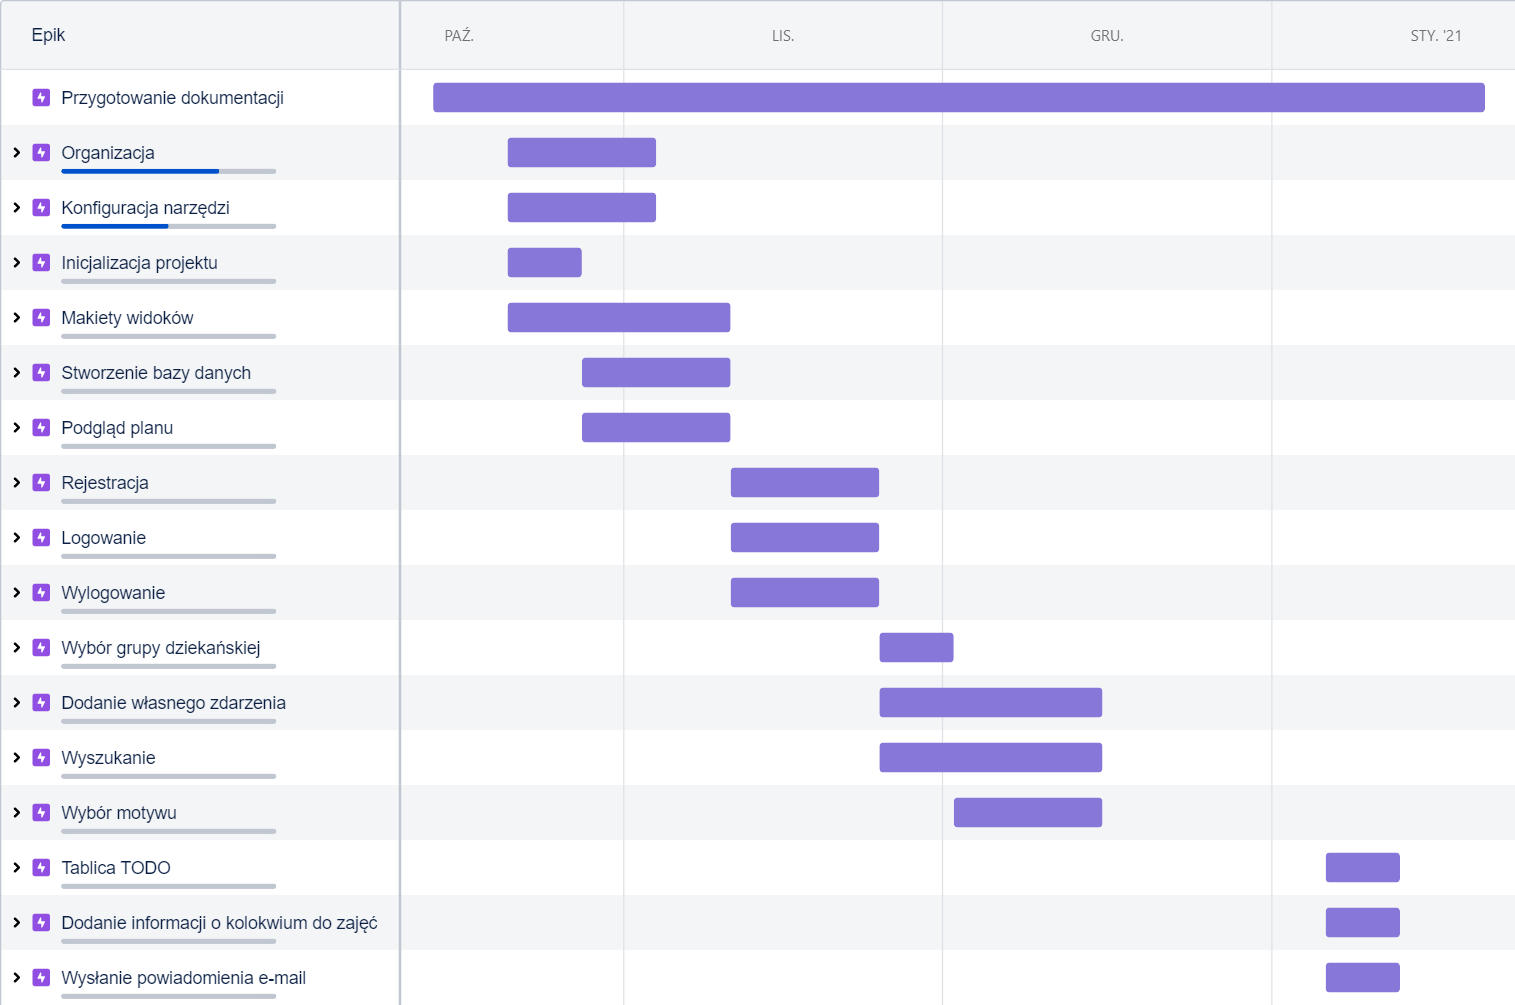
\includegraphics[width=0.85\textwidth]{pictures/fabulous_uz_planner_2020-10-27_06.13pm.png}
        \caption{Diagram Gantta}
	\vspace{-30pt}
     \end{figure}

\begin{center}
\begin{tabular}{ |m{6cm} | m{3cm}| m{3.5cm} | m{3cm} | } 
\hline
\textbf{Zadanie} 					& \textbf{Stanisław Mól} 	& \textbf{Mateusz Znojek} 		& \textbf{Erwin Konkel} \\ 
\hline
Przygotowanie dokumentacji 			& \checkmark			& 						&  \\ 
\hline
Organizacja 						& \checkmark 			& \checkmark 				& \checkmark \\ 
\hline
Konfiguracja narzędzi 					& \checkmark 			& \checkmark 				& \checkmark \\ 	
\hline
Inicjalizacja projektu					& \checkmark 			&  		 				&   \\ 
\hline
Makiety widoków					& 					&  		 				& \checkmark \\ 
\hline
Stworzenie bazy danych 				& 					& \checkmark 				&   \\ 
\hline
Podgląd planu 						& \checkmark 			&  		 				&   \\ 
\hline
Rejestracja 						& 					& \checkmark 				&   \\ 		
\hline
Logowanie 						& 					&  		 				& \checkmark \\ 
\hline
Wylogowanie 						&  					& \checkmark 				&   \\ 
\hline
Wybór grupy dziekańskiej 				&  					&  		 				& \checkmark \\ 
\hline
Dodanie własnego zdarzenia 			&  					& \checkmark 				&   \\ 
\hline
Wyszukiwanie 						& \checkmark 			&  		 				&   \\ 
\hline
Wybór motywu 						& 					& 		 				& \checkmark \\ 
\hline
Tabica TODO 						&  					& \checkmark 				&   \\ 
\hline
Dodanie informacji o kolokwium do zajęć 	& \checkmark 			& 		 				& \checkmark \\ 
\hline
Wysłanie powiadomienia e-mail 			& \checkmark			& \checkmark				& \checkmark \\ 
\hline
\end{tabular}
\end{center}

\clearpage
\section{Plan testów}
	Plan testów zakłada testowanie każdej historyjki przed oddaniem jej. Oznacza to, że każda funkcjonalność powinna zostać przetestowana przed dodaniem jej do głównej gałęzu projektu. Testy powinny być przeprowadzone na podstawie wyznaczonych kryteriów akceptacji.

\section{Plan bezpieczeństwa}
	Plan bezpieczeństwa zakłada dostarczenie możliwie uniwersalnych mechanizmów dla:
            \begin{itemize}[leftmargin=0.5in]
                \item uwierzytelniania (ang. authentication) - jestem tym za kogo się podaję bo: znam pin, znam hasło, mam takie odciski palców, posiadam certyfikat 			SSL, itp.
                \item autoryzacji (ang. authorization) - mam dostęp do określonych zasobów, a do innych nie
            \end{itemize}

    \begin{figure}[ht!]
        \centering
        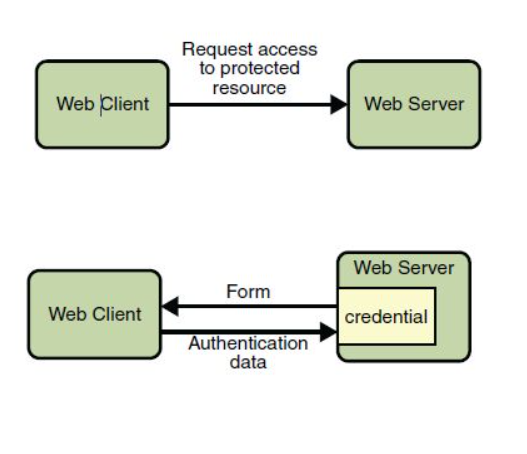
\includegraphics[width=6in]{pictures/uwierzytelnianie_klienta_web.png}
        \caption{Uwierzytelnienie klienta web}
        \label{fig10}
     \end{figure}

\section{Plan konserwacji}

Plan konserwacji obejmuje weryfikację oraz poprawanie błędów w trakcie implementacji każdej z nowych funkcjonalności. Po zakończeniu projektu, nie sa planowane kolejne aktualizacje.

\section{Warunki licencji}

    Planneruz jest wolnym oprogramowaniem: możesz go rozprowadzać dalej
    i/lub modyfikować na warunkach Powszechnej Licencji Publicznej GNU,
    wydanej przez Fundację Wolnego Oprogramowania - według wersji 3 tej
    Licencji.\\

    Planneruz rozpowszechniany jest z nadzieją, iż będzie on
    użyteczny - jednak BEZ JAKIEJKOLWIEK GWARANCJI, nawet domyślnej
    gwarancji PRZYDATNOŚCI HANDLOWEJ albo PRZYDATNOŚCI DO OKREŚLONYCH
    ZASTOSOWAŃ. W celu uzyskania bliższych informacji sięgnij do Powszechnej Licencji Publicznej GNU.\\

    Z pewnością wraz z Planneruz otrzymałeś też egzemplarz
    Powszechnej Licencji Publicznej GNU (GNU General Public License).
    Jeśli nie - zobacz http://www.gnu.org/licenses.\\

\end{document}

